\section{Perforator первой версии}
В рамках данной работы проводилась разработка системы распределенного анализа производительности приложений на масштабах целых датацентов.
Система носит рабочее название <<Perforator>>.

\subsection{Архитектура}
В начале разработки требовалось за наиболее короткое время получить рабочий прототип,
позволяющий регулярно собирать актуальные профили с промышленных окружений и проводить
оптимизации реальных программ. Для решения была выработана следующая архитектура:

\begin{itemize}
    \item
        Централизированный микросервис <<Scraper>> получает профили с заранее настроенного списка сервисов.

    \item
        Каждый полученный профиль аннотируется дополнительными метками, такими как имя хоста и модель CPU, после чего записывается в общее хранилище профилей.

    \item
        Хранилище профилей реализовано поверх широко используемой внутри Яндекса системы хранения и обработки данных YTsaurus \cite{yt}.

    \item
        Для изучения профилей разработчиками был написан достаточно примитивный веб-интерфейс, позволяющий смотреть список профилей
        в порядке появления по конкретным сервисам и по всей системе.

    \item
        Профили регулярно удаляются из системы: разработчикам интересны актуальные профили.
        При этом, поддержана возможность сохранять некоторые профили (те, что изучали разработчики) на значительно большее время.

    \item
        В настоящее время в системе не поддержана агрегация профилей по различным измерениям.
        Например, нельзя построить профиль по всему сервису за день или профиль по конкретному хосту.

\end{itemize}

Рассмотрим основные компоненты системы подробнее.

\begin{figure}[H]
    \centering
    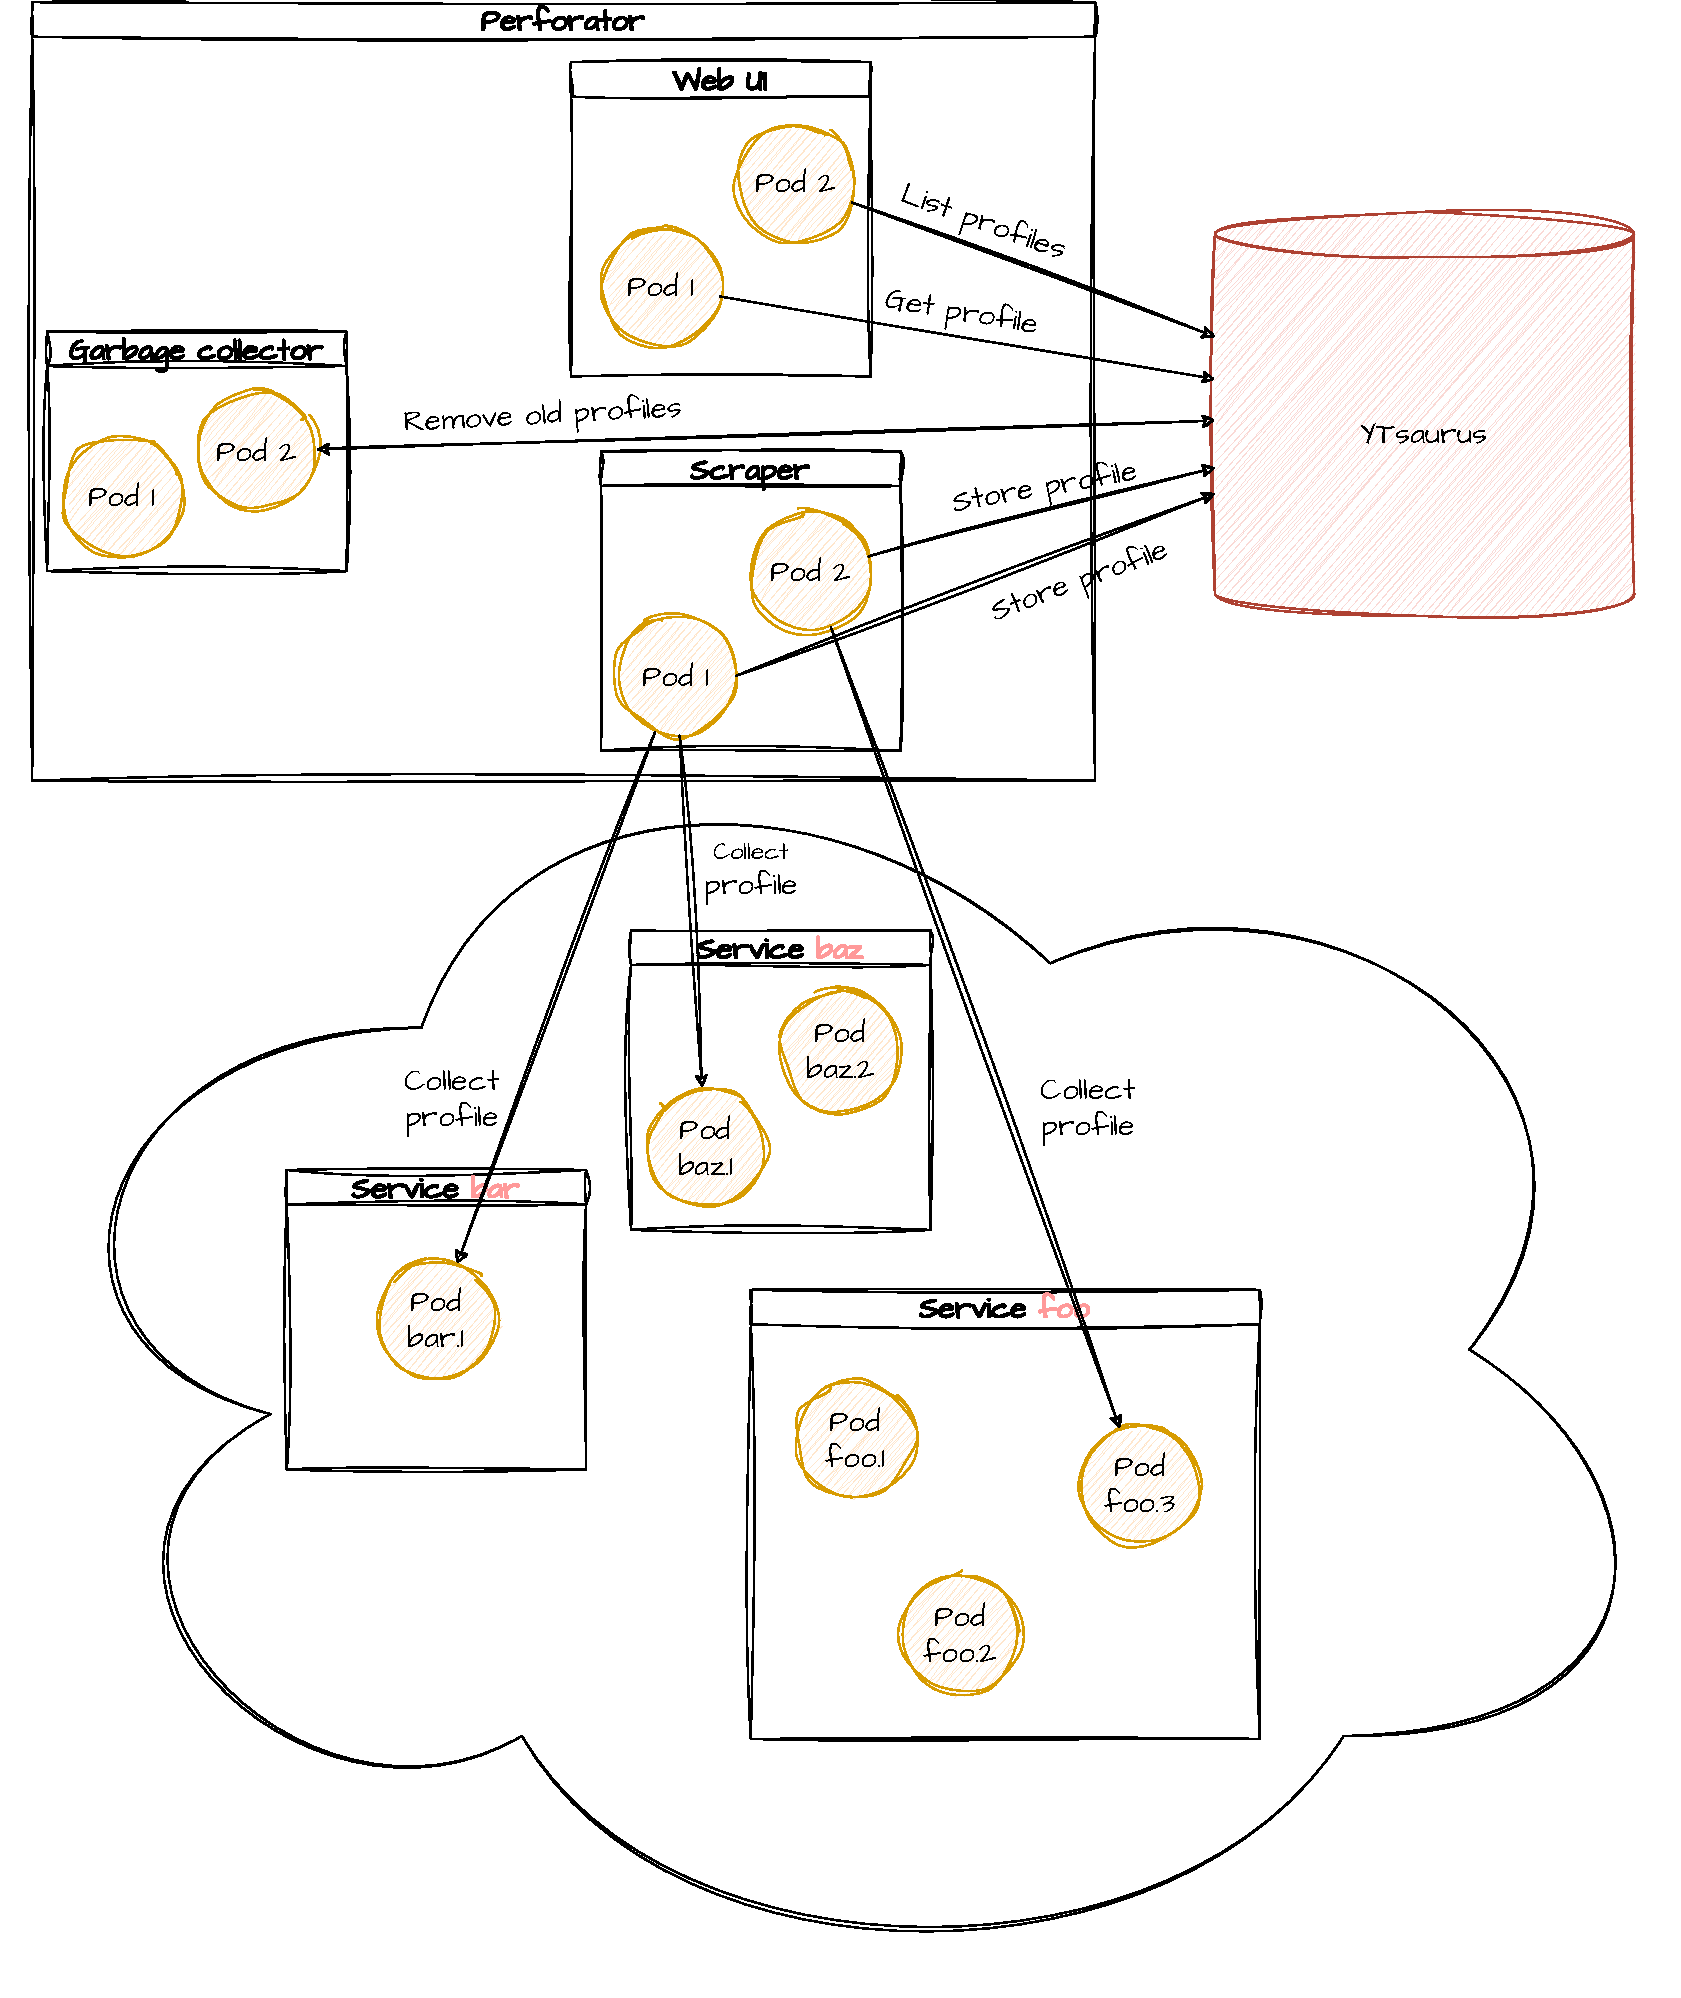
\includegraphics[width=\textwidth]{perforator.pdf}
    \caption{Схема первой версии сервиса}
    \label{fig:simple}
\end{figure}

\subsubsection{Сборщик профилей}
Scraper проходится по каждому сервису, подключается к нему одним из поддержанных способов (по HTTP, через SSH) и собирает профиль.
В настоящее время основным способом подключения сервиса является настройка доступа Scraper к хостам сервиса через SSH.
В этом режиме Scraper использует perf для сбора профиля по CPU cycles.
После сбора профиля на каждом хосте perf символизирует профиль, превращая адреса инструкций в имена функций.
Результат работы perf конвертируется в формат pprof: стандартный для большого количества современных семплирующих профилировщиков
формат, используемый в pprof и gperftools.

Подавляющее большинство сервисов, анализируемых Scraper, запущены в контейнерах под управлением системы контейнеризации Porto \cite{porto}.
Scraper анализирует конкретные процессы, определяемые по заданным пользователями правилам:
например, слушающие на определенном TCP порту или имеющим строку запуска, удовлетворяющую регулярному выражению.

Типичное время сбора профиля – минута на частоте около 500 Hz (десятки тысяч семплов), типичный размер сжатого профиля – 5 MiB.
В теории сервис не ограничен видом анализируемой метрики, профили могут быть произвольной природы.
В частности, тривиально поддерживются различные виды системных метрик, доступных подсистеме Linux perf.
На практике подавляющее большинство профилей собирается семплированием тактов процессора.

По результатам анализа не было выявлено сколько-нибудь значимого эффекта при включении perf на продуктовых процессах,
включая самые чувствительные к задержкам.

Для защиты от потенциальных проблем Scraper анализирует не все хосты сервиса, а небольшое статически выбираемое подмножество.
Это позволяет гарантировать, что в случае проблем с реализацией Perforator, perf или ядра Linux профилирования не нанесет значительного
вреда сервису.

Благодаря pull модели (сервис сам забирает профили с системы), автоматически поддержана возможность собирать профили с встроенных
в программу библиотек профилирования, таких как \lstinline!net/http/pprof! \cite{golang:pprof} в Golang.

\subsubsection{Хранилище профилей}
Хранилище профилей реализовано поверх широко используемой внутри Яндекса системы хранения и обработки данных YTsaurus \cite{yt}.
Хранилище разбито на две \textit{динамических таблицы} (OLTP KV хранилище в терминах YTsaurus).

Легковесная таблица метаинформации хранит нужную для обработки и поиска информацию о профиле: с какого хоста он снят, в какое время.
Данная таблица находится целиком в памяти, доступ к ней дешевый и эффективный,
это позволяет использовать тяжелые full-scan запросы при работе с ней.

Тяжелая таблица профилей содержит собственно профили, запросы туда исключительно легкие для системы: выбор профиля по ключу
(LookupRows в терминах YTsaurus). Кроме того, вместо данной таблицы поддержана возможность организации хранилища при помощи
Amazon S3-совместимого провайдера.
В этом режиме использование специализированной для хранения тяжелых данных системы позволяет сэкономить диск и снизить расходы
на чтение и запись профилей. При использовании динамических таблиц тяжелые профили неизбежно проходят через протокол консенсуса.

\subsubsection{Визуализация}
Для изучения профилей разработчиками был написан достаточно примитивный веб-интерфейс с использованием
UI-фреймворка Bootstrap \cite{bootstrap}, позволяющий смотреть список профилей
в порядке появления по конкретным сервисам и по всей системе.
Профили визуализируются в формате Flamegraph.

При разработке сервиса был реализован код отрисовки flamegraph, так как оригинальный код Brendan Gregg \cite{flamegraph}
не отличался большой производительностью: на отрисовку flamegraph по одному профилю в несколько мегабайт тратилось несколько минут.
Скрипт был переписан на Golang и дополнительно оптимизирован, что позволило ускорить отрисовку в десятки раз.

Кроме того, было найдено несколько ошибок в данном крайне популярном инструменте, один из которых был критичным.
При анализе результата работы perf flamegraph не учитывал веса семплов.
Это приводило к появлению на профиле большого количества (вплоть до 30\%) функций переключения контекста в ядре операционной
системы. При переключении контекста необходимо обновить состояние PMU, и современные процессоры при переключении
генерируют большое количество прерываний с нулевым весом.

Данная проблема была найдена несколькими независимыми разработчиками.
Стороннее решение появилось \cite{flamegraph:weight} вскоре после обнаружения в данном проекте.

\subsubsection{Сборка мусора}
Профили регулярно удаляются из системы: разработчикам интересны актуальные профили.
Выбрана экспоненциально затухающая политика хранения профилей с настраиваемым периодом полураспада профиля.
При этом, поддержана возможность сохранять некоторые профили (те, что изучали разработчики) на значительно большее время.

\subsubsection{Продвинутые возможности}
Система поддерживает возможность анализа конкретного хоста сервиса по запросу пользователя.
Это позволяет точечно анализировать проблемые хосты, не дожидаясь, пока Scraper случайным образом выберет их.

\subsection{Внедрение}
Первая версия системы была разработана и внедрена в сжатые сроки.
Легкий доступ к большому количеству актуальных профилей позволил разработчикам быстро устранять узкие места,
что привело к суммарному объему оптимизаций порядка десятков тысяч процессорных ядер.
Экспериментально было подтверждено эмпирическое наблюдение, что профиль программы под нагрузкой часто сильно отличается от профиля в
спокойном состоянии. Для некоторых сервисов различие настолько велико, что для оптимизации пропускной способности имеет
смысл рассматривать исключительно предкритическое состояние под нагрузкой.

\subsection{Ограничения}
Описанная система отличается простотой реализации, что неизбежно приводит к значительным ограничениям:

\begin{itemize}
    \item
        Одной из самых больших проблем является необходимость ручной настройки системы для каждого сервиса.
        Владелец сервиса должен выдать доступ Scraper по SSH и явно прописать свой сервис в конфигурации Perforator.

    \item
        Использование perf в качестве основного инструмента профилирования приводит к не менее серьезным ограничениям.
        Все анализируемые сервисом программы должны быть собраны с директивой компилятора, запрещающим опускать пролог и эпилог функций.
        Это позволяет быстро раскручивать стеки через perf, однако требует нетривиальной настройки со стороны владельцев сервисов, и,
        потенциально, приводит к потери производительности.

        В качестве альтернативы пользователи могут включать особые режимы сбора стеков через perf: с использованием
        DWARF (см. \ref{sec:dwarf}) или LBR (см. \ref{sec:lbr}).
        К сожалению, оба механизма недостаточно хорошо показывают себя на реальных задачах.
        Раскрутка через DWARF крайне тяжелая (каждый семпл копирует большой регион стека процесса из kernel space в user space).
        Оба варианта работают эвристически и часто теряют функции у основания стека из-за большой глубины стека в реальных программах
        (десятки и сотни функций).

    \item
        В настоящее время в системе не поддержана агрегация профилей по различным измерениям.
        Например, нельзя построить профиль по всему сервису за день или профиль по конкретному хосту.

    \item
        Pull схема плохо масштабируется. Scraper должен знать список всех серверов, где необходимо собирать профили.
\end{itemize}

С учетом вышеописанных проблем было принято решение о разработке значительно более сложной системы, призванной решить
все сложности простой схемы.

\section{Yandex-wide Perforator}
\subsection{Требования}
После анализа существующих решений и известных проблем первой версии Perforator были выделены следующие требования к системе:
\begin{itemize}
    \item
        Профилировщик должен поддерживать максимально точную раскрутку стеков.

    \item
        Все сервисы и серверы, находящиеся во внутреннем облаке Яндекса, должны подключаться к системе без участия администраторов.
        Это позволит получить точные профили всего флота компании, не требуя внимания и ручных действий от пользователей.

    \item
        Должна поддерживаться возможность получить значения локальных для потока переменных.
        Это позволит реализовать профилирование по конкретным A/B экспериментам, как сделано в \ref{sec:yabs}.

    \item
        Профилировщик не должен влиять на анализируемые процессы.
        Например, ожидаемая просадка производительности от включения профилировщика не должна превышать одного-двух процентов CPU.

    \item
        Должна поддерживаться как и push-схема, так и pull.
        Для некоторых типов профилировщиков имеет смысл оставить первую версию системы, например, для встроенного в Golang профилировщика.
        Более того, некоторые пользователи хотят иметь возможность заливать собранные своим способом профили в систему.
\end{itemize}

\subsection{Архитектура}
Была выбрана следующая архитектура:
\begin{itemize}
    \item
        На каждом сервере, принадлежащему общему облаку Яндекса, будет запущен агент Perforator.
        Агент будет наблюдать за контейнерами сервисов на данном сервере.
        Агент настраивает PMU через \verb!perf_event_open!, после чего подключает eBPF программу для раскрутки стека и анализа
        состояния наблюдаемых процессов через \verb!PERF_EVENT_IOC_SET_BPF!: механизм, вызывающий eBPF программу на каждое прерывание от PMU.
        Агент собирает по 99 семплов с каждого процессорного ядра в секунду.

    \item
        Агент регулярно (сейчас --- раз в минуту) отправляет собранные профили в формате pprof в хранилище.
        В отличие от первой версии Perforator, система не знает про список сервисов и хостов: реализована push-схема.

    \item
        Хранилище профилей реализовано как развитие хранилища в первой версии.
        В настоящее время активно разрабатывается агрегация профилей, однако пока еще финальной версии не реализовано.

    \item
        В отличие от первой версии, профили в систему попадают не символизированные.
        С учетом большого количества реплицированных сервисов, локальная символизация на агентах признана неэффективной.
        Например, существуют сервисы, имеющие множество одинаковых реплик на разных серверах.
        В случае локальной символизации придется символизировать похожие профили тысячи раз на разных репликах.
        При этом намного эффективнее собрать все профили со всех реплик сервиса в одном месте, после чего символизировать вместе,
        переиспользуя кеши символизатора.
\end{itemize}

\subsubsection{Агент}
В реализации рассматриваемой системы наиболее сложной компонентой является агент.
Агент должен эффективно взаимодействовать с ядром Linux, не оказывая заметного влияния на систему.

Агент выполняется с правами суперпользователя; более точно, для работы агента требуется capability \verb!CAP_SYS_ADMIN!.
Данные права позволяют иметь полный доступ до всех компонент системы, что, к сожалению, необходимо при использовании
подсистем eBPF и perf.

Агент реализует раскрутку стеков через eBPF программу.
В рамках разработки Perforator была решена задача раскрутки стеков с использованием DWARF CFI в пространстве ядра,
что позволяет не включать спорную опцию \verb!-fno-omit-frame-pointer! на всю компанию.

\subsubsection{eBPF программа}
Когда агент обнаруживает новый контейнер (cgroup), он открывает файловый дескриптор для мониторинга производительности через
\verb!perf_event_open! и подключает к нему eBPF программу.
eBPF программа выполняется каждый раз, когда переполняется PMU счетчик (обычно счетчик количества циклов процессора).
Это позволяет семплированно с определенной частотой собирать информацию об использовании циклов процессора различными процессами в системе.
Агрегация собранных семплов позволяет получить приблизительный профиль использования CPU различными функциями процессов.

Благодаря тому, что минимальная поддерживаемая Perforator версия Linux --- 5.4, агент может использовать
достаточно сложную eBPF программу. В частности, на каждый семпл собираются следующая информация:
\begin{itemize}
    \item
        ID процесса и потока, имя потока, время старта процесса.
        Это позволяет уникально идентифицировать потоки; одних идентификаторов недостаточно, так как их количество достаточно сильно
        ограничено, и PID достаточно часто переиспользуются в системе.

    \item
        Количество событий, произошедших с момента прошлого прерывания.
        При сборе данной метрики необходимо учитывать проблему мультиплексирования PMU:
        количество регистров PMU на процессоре ограничено, и если параллельно с агентом на машине выполняются другие инструменты
        анализа производительности при помощи PMU, то система будет с высокой частотой включать и выключать регистры агента на PMU.
        Это приводит к проблеме потери семплов: если, например, запустить несколько агентов на одной машине, то
        каждый из них получит кратно меньше прерываний.
        К счастью, ядро позволяет получить отношение времени, когда регистры агента были активны на
        PMU к количеству времени, когда регистры агента были настроены.
        Домножая общее количество событий на данную долю активного времени можно получить оценку на реальное количество произошедших
        событий.

        К примеру, если PMU сообщает, что с последнего прерывания произошло 1000 циклов, при этом регистры агента были активны 80\% времени,
        то реальное количество циклов равно 1250.

    \item
        Стек вызовов в ядре, если прерывание произошло в контексте ядра.
        Это позволяет отлаживать проблемы производительности не только в пользовательском пространстве.

    \item
        Стек вызовов в пространстве пользователя.
        Стек вызовов раскручивается с использованием оптимизированной DWARF CFI по методике, описанной ниже.

    \item
        Идентификатор cgroup процесса.
        Наличие данного идентификатора позволяет понимать, к какому контейнеру следует засчитывать собранные семплы.
\end{itemize}

eBPF программа записывает собранные семплы в perf event buffer ровно таким же механизмом, которым вышеописанный perf
записывает собранные семплы в кольцевой буфер.

\subsubsection{Раскрутка стеков}
Раскрутка стеков с использованием DWARF CFI в пространстве ядра стала возможна благодаря следующему наблюдению.
Хоть DWARF CFI и поддерживают таблицы раскрутки привольной сложности (см. \ref{sec:dwarf}),
на практике компиляторы генерируют крайне простые инструкции, не используя Тьюринг-полные возможности CFI.

Для подтверждения гипотезы был рассмотрен большой (более 3000) набор бинарных файлов архитектуры x86-64,
полученных из нескольких разных источников:
\begin{itemize}
    \item Бинарные файлы из популярных пакетов Ubunbu Linux, Fedora Linux и Arch Linux
    \item Статически собранные оптимизированные бинарные файлы из внутреннего облака Яндекса.
\end{itemize}
При анализе различные строки FDE классифицировались на принадлежность нескольким известным классам CFI инструкций, после чего
подсчитывалась общая статистика.

Были получены следующие результаты:
\begin{itemize}
    \item
        Для вычисления CFA на x86-64 в 99.340\% строк FDE достаточно правила \verb!%rsp + const!,
        где const --- небольшое (меньше 8 бит) число.
        Компиляторы генерируют предсказуемый код, редко изменяя стековый регистр.
        Еще в 0.636\% случаев CFA вычисляется как \verb!%rbp + const!.
        Встречется несколько уникальных правил раскрутки, написанных руками, например, в OpenSSL, однако
        реально таких правил единицы, и их легко реализовать в eBPF.

    \item
        С учетом первого результата значительный интерес вызывает поддержание актуального состояние регистра \verb!%rbp! при раскрутке.
        Регистр восстановим при раскрутке не всегда, в 56\% случаев это невозможно; однако остальные
        случаи всегда описываются одним тривиальным правилом: \verb!*(cfa - const)!, где const --- небольшая константа, кратная 8.
        Опять же, полученный результат легко объяснить: \verb!rbp! --- calle-saved регистр, и каждая нетривиальная функция в первую очередь
        сохраняет состояния calle-saved регистров в начале своего стекового кадра.

    \item
        Ожидаемым образом, для раскрутки адреса возврата на x86-64 в 100\% случаев достаточно прочитать 8 байт перед CFA: \verb!*(cfa + 8)!.
        Вход в функции реализуется инструкцией call, которая записывает адрес возврата на стек и уменьшает стековый указатель на 8 байт.
\end{itemize}

С учетом обнаруженных особенностей можно реализовать достаточно простой алгоритм
точной раскрутки стека без использования frame pointers.

Более того, при раскрутке стека алгоритм поддерживает три регистра: \verb!rsp!, \verb!rbp! и \verb!rip!.
Важно, что тех же регистров достаточно для раскрутки стека через frame pointers; оказывается, что мы можем реализовать
алгоритм смешанной раскрутки одновременно через DWARF CFI и frame pointers, пропуская анализ DWARF CFI для тех функций, что содержат
frame pointers.

В частности, данный алгоритм успешно реализован в eBPF программе агента Perforator, позволяющей раскручивать стеки глубиной до 256 вызовов.
Скорее всего, данный лимит можно значительно повысить вплоть до нескольких тысяч вызовов.
При реализации алгоритма было обнаружено несколько сложностей:
\begin{itemize}
    \item
    Для раскрутки через DWARF CFI eBPF программе необходимо иметь доступ до проанализированных таблиц DWARF.
    Данный анализ невозможно выполнить в пространстве ядра хотя бы потому, что нужных для анализа страниц исполняемого файла может не
    оказаться в памяти, а eBPF программы не имеют возможности взаимодействовать с блочными устройствами (дисками).

    В Perforator доставка таблиц раскрутки решена следующим образом.
    eBPF программа при обнаружении нового процесса (при получении первого семпла этого процесса) уведомляет
    агент в пользовательском процессе через запись соответствующего события в кольцевой буфер.
    Агент анализирует состояние процесса, вычитывает его файловые отображения для поиска исполняемых файлов и динамических библиотек,
    после чего при помощи вспомогательной программы с использованием инструментария анализа исполняемого кода, доступного в LLVM \cite{llvm},
    генерирует сжатые таблицы раскрутки.

    Размер таблиц раскрутки крайне мал. Для самых больших бинарных файлов на 1GiB секции с кодом \verb!.text!
    размер таблицы составляет 9M строк, что в сжатом при помощи zstd \cite{zstd} состоянии занимает около 5MiB.

    После анализа таблиц раскрутки агент регистрирует их в eBPF отображении, доступном eBPF программе.
    Как только программа получает новый семл, принадлежащий проанализированному процессу,
    она переключается с раскрутки с использованием frame pointers на смешанную раскрутку с использованием DWARF CFI.

    \item
    При раскрутке через DWARF CFI eBPF программа бинарным поиском по адресу инструкции находит подходящую строку.
    Бинарный поиск здесь --- наиболее сложная часть eBPF программы для анализа верификатором.
    Было найдено несколько достаточно серьезных проблем при использовании верификатора в ядрах версии Linux 5.4.
    В частности, верификатор не поддерживает анализ сложных вложенных циклов.
    Агент при раскрутке использует цикл следующего вида:
    \begin{verbatim}
    for (int i = 0; i < DWARF_MAX_STACK_DEPTH; ++i) {
        // one step of the unwinder
        for (int j = 0; j < MAX_BINARY_SEARCH_STEPS; ++j) {
            // find matching unwind table row for the given rip
            ...
        }
    }
    \end{verbatim}
    верификатор отвергает данный цикл с ошибкой <<infinite loop detected>>.
    Анализ исходного кода Linux показал, что причиной ошибки стала ограниченная возможность верификатора отслеживать
    выполнение циклов, в какой-то момент сохраняющих регистр счетчика итераций на стек (register spilling).
    Верификатор для отслеживания корректности программы поддерживает множество состояний --- наборов классов значений регистров.
    В этих состояниях не учитываются возможные сохраненные на стек регистры \cite{bpf:loop}, поэтому при итерации
    верификатор получал два одинаковых состояния и считал, что цикл бесконечен.

    Решением данной проблемы стало использование вложенных функций в eBPF (bpf to bpf calls, новая возможность из Linux 4.16).
    При использовании функций верификатор хранит намного больше контекста в одном состоянии (по числу вложенных вызовов функций).
    После выделения вложенного цикла в отдельную функцию верификатор получил возможность отслеживать точные состояния циклов \cite{bpf:func}.

    \item
    Perforator недостаточно хорошо обрабатывает короткоживущие процессы.
    Например, если процесс завершается за несколько миллисекунд, то с большой вероятностью агент не успеет вычитать событие с семплом
    от eBPF программы за время, пока процесс жив.
    Так как анализ семплов требует некоторой информации об процессе, откуда был получен семпл, такие семплы оказываются недостаточно полными
    и теряются.

    Для символизации сырых адресов необходимо знать, какому исполняемому файлу и какой позиции соответствует в нем
    заданная инструкция. К сожалению, для небольшого количества семплов Perforator не имеет возможности получить информацию об
    отображении виртуального адреса в исполняемый файл (например, по причине описанных выше короткоживущих процессов).
    Такие семплы оказываются в системе без возможности быть символизированными.

    Практика использования агента Perforator показывает, что на различных серверах теряется от 1\% до 5\% семплов.
    Мы расцениваем такой результат положительно, так как выводы об производительности по оставшимся 95\% семплов будут достаточно
    обоснованнные.

    \item
    Perforator в настоящее время не поддерживает программы, использующие по одному и тому же виртуальному адресу
    разные файловые отображения исполняемых файлов.
    Это ограничение вызвано архитектурой взаимодействия eBPF программы с агентом: нельзя гарантировать, что при изменении отображения
    программа вовремя обнаружит правильную версию таблицы раскрутки.
\end{itemize}

\subsubsection{Символизатор}
Существенным отличием новой версией системы стало наличие отдельного символизатора.
Символизатор вычитывает сырые профили из хранилища, ищет подходящие бинарные файлы,
превращает сырые адреса в список функций, имен исходных файлов и номеров строк при помощи инструментария LLVM
и записывает полученный символизированный профиль обратно в систему.

Самым нетривиальным этапом при символизации является поиск исполняемых файлов.
Для решения этой задачи было разработано выделенное хранилище бинарных файлов.
Агенты, общаясь с сервисом Perforator, сообщают ему список известных агентам бинарных файлов и получают указания
о загрузке некоторых файлов с серверов в систему Perforator.
Далее эти бинарные файлы используются символизатором.

Для уникальной идентификации файлов используется механизм BuildID.
BuildID --- особая секция в ELF файлах, хранящая подсчитанный при компановке криптографический хеш от исполняемых секций файла.
BuildID позволяет уникально идентифицировать исполняемые файлы на всех уровнях системы.

К сожалению, не все программы содержат секцию с BuildID.
На серверах с агентом Perforator примерно 10\% файлов не содеражат этого идентификатора.
Для решения этой проблемы Perforator вычисляет крайне простой идентификатор для таких бинарных файлов,
детерминировано выбирая несколько 30 произвольных страниц из исполняемых секций и считая хеш от этих страниц.
Данный подход позволяет значительно сэкономить время по сравнению с вычислением классического BuildID.

\subsubsection{Контекст потока}
Для поддержки анализа A/B экспериментов в Perforator был продуман дизайн решения, позволяющего в eBPF программе вычитывать состояние
локальных для потока переменных.
Для этого планируется разработка библиотеки, поддерживающей несколько типов тред-локальных переменных и
инициализирующих их особым образом (записью магического числа по умолчанию).
Начальные значения локальных для потока переменных, как и их смещения внутри локального региона памяти потока (thread local storage),
хранятся в отдельной секции ELF.
Perforator сможет поддерживать чтения этих переменных для определенного набора платформ (musl, glibc) и
архитектур (x86-64). Для этого агент при анализе новых исполняемых файлов будет искать заданные магические константы
(заранее сгенерированные псевдослучайные числа) в данной секции.

\subsection{Разработка}
Perforator активно разрабатывался на протяжении нескольких месяцев.
На момент написания отчета, Perforator содержит порядка 15000 строк исходного кода на Go (агент, хранилище),
C++ (символизатор, анализатор табилц раскрутки) и C (eBPF программы).

\subsection{Тестирование}
Агент Perforator тестируется обширным набором unit-тестов, а так же покоммитными проверками работоспособности агента на разных версиях
ядра Linux при помощи QEMU \cite{qemu}.

\subsection{Внедрение}
Первая версия Perforator полностью внедрена и активно используется.
Новая версия Perforator активно внедряется в настоящее время, основные компоненты разработаны и протестированы.
Можно ожидать полноценного внедрения летом 2023.

При анализе замедления производительности от использования агента Perforator не было найдено сколько-нибудь значимых эффектов.
Можно ожидать не более одного процента просадки производительности.
